\documentclass[11pt]{article}

\usepackage{fullpage}
\usepackage{graphicx}

\begin{document}

\title{ARM11 Final Report}

\author{Aahil MEHTA, Miroslav LAMBREV, Radostin PETROV, Ruari PHIPPS}

\maketitle

\section{ARM11 emulator and assembler}
\begin{minipage}{0.6\linewidth}
\subsection{Emulator implementation}

For initial implementation of the emulator, check \texttt{doc/Checkpoint.tex}. We have since modified the emulator by introducing a \texttt{decode.c} module, that depends on a \texttt{decode.h} header, which serves to process and decode the different types of instructions. That way we have split the work done by \texttt{execute.c} roughly in half and spread it between it and \texttt{decode.c}. The dependency graph for the emulator has since slightly changed.

\subsection{Assembler implementation}

Our assembler has the following structure:
\begin{itemize}
    \item The \texttt{assemble.c} file contains the \texttt{process\_instruction} function, which is a helper function to \texttt{main}, uses a look up table to find out what type of instruction we are dealing with it and return the appropriate parse function for it. The \texttt{main} function takes the incoming assembly file and the output binary filename as arguments. It then opens the file for reading and creates the symbol table, opcode table and the parse type table. Then we start the two-pass structure, the first pass being the symbol table generation by analyzing the file line by line. In the second pass we generate the binary encoding for each instruction and then write it into memory. After that has been successfully done, we save the memory into a file with a name given by the second argument.
    \end{itemize}
    \end{minipage}
\hspace{0.05\linewidth}
\begin{minipage}{0.35\linewidth}

\centering

\includegraphics[scale=0.8]{diagrams/EmulatorDependences.png}
\caption{Figure 1: Dependency Diagram for \texttt{emulate.c}}

\end{minipage}
    \begin{itemize}
    \item The \texttt{parser.c} file has all the parsing functions for all types of instructions (special included), as well as functions to parse the register and the expressions (in the case of immediate values).
    \end{itemize}
\begin{minipage}{0.6\linewidth}
    \begin{itemize}
    \item \texttt{assembler\_utils.c} contains utility functions that we use in the assembler, such as functions to move an instruction, to generate the offset in branch instructions, writing to memory and saving the memory into output file.
    \item The \texttt{symbol\_table.c} file has all functions connected to our \texttt{Symbol\_Table} struct, defined in \texttt{symbol\_table.h}. These include functions for initializing the table, adding entries and creating the opcode and parse type tables, which also utilize the same struct.
\end{itemize}
\par For all of the \texttt{.c} files in our implementation (except \texttt{assemble.c}) we have their respective header file, containing the dependent libraries.
\end{minipage}
\hspace{0.05\linewidth}
\begin{minipage}{0.35\linewidth}

\centering
\vspace{5mm}
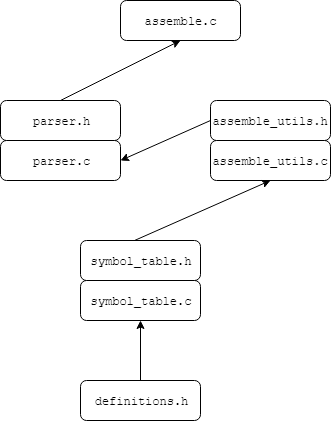
\includegraphics[scale=0.8]{diagrams/AssemblerDependencies.png}
\caption{Figure 2: Dependency Diagram for \texttt{assemble.c}}

\end{minipage}

\subsection{General purpose IO on a Raspberry Pi}
We initially extended \texttt{emulate.c} and \texttt{assemble.c} to support the gpio functions and after we successfully passed the tests we tested in successfully on the Raspberry Pi. \texttt{/programs/gpio.s} contains the assembly code we used for this part.

\subsection{Testing ?}

\vspace{4mm}

\section{C120.3 Extension: Game Engine}
\end{document}
